Photoelectron multiplier tube, PMT, employed as photosensors in nuclear physics during decades, detect the scintillating photons that reach its sensitive part, photocathode, and produce an electronic signal, large enough to be easily measured. In Figure \ref{fig:SchemePMT} a schematic drawing of a PMT is given. The PMT consists of a vacuum tube that has a glass window through which photons can penetrate. The electrons created in the photocathode travel in vacuum. 

\begin{figure}[htbp]
\centering
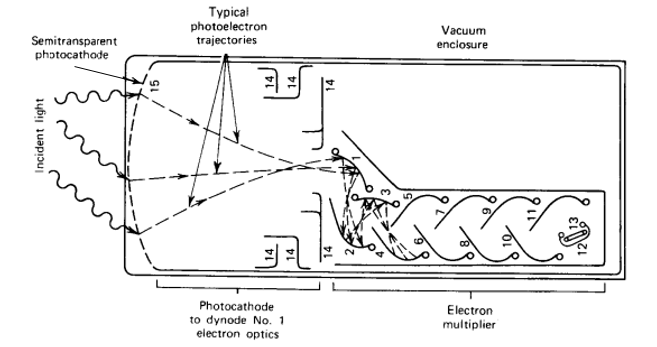
\includegraphics[scale=0.6]{3DesignPrinciples/32Tritium_detector/PMTschematic.png}
\caption{Scheme of a PMT.\label{fig:SchemePMT}~\cite{Knoll}}
\end{figure}

The signal production has two phases:

\begin{enumerate}
\item{} In the photoathode photons are converted in photoelectrons through photoelectric effect. The photocathode consists of a thin layer, of the order of nanometers, deposited on the inner surface of the PMT window. The material of the photocathode is chosen to optimize the probability of producing photoelectric effect with the scintillating photons. The PMTs used in TRITIUM experiment are the model R8520-406 from Hammatsu \cite{DataSheetPMTs} and the material of their photocathode is Bialkali\footnote{The bialkali material is based on the elements $\ce{^{121}_{51}Sb}$, $\ce{^{85}_{37}Rb}$ and $\ce{^{132}_{55}Cs}$}.

The response of the PMT at long wavelengths is limited mainly because photon energy is not enough to produce a photoelectric effect or the emitted photoelectron does not have enough energy to overcome the material-work function. The response of the PMT at short wavelengths is limited due to absorption in the window material, quartz in our case. THus, the response of the PMT has a strong dependence on the energy of the photon and the quantum efficiency (QE)  spectrum defined is given by the ratio of the number of photoelectrons produced at the cathode of the PMT and the number of photons reaching it. For PMTs used in the TRITIUM experiment, the QE is showed in Figure \ref{fig:QuantumEfficiencyPMT}.

\begin{figure}[htbp]
\centering
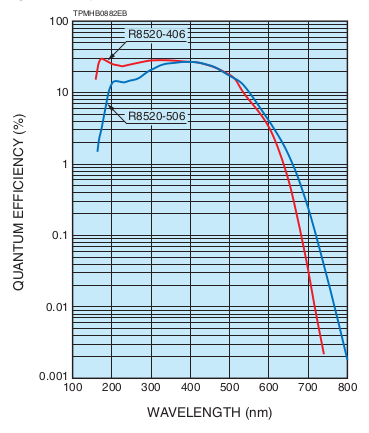
\includegraphics[scale=0.5]{3DesignPrinciples/32Tritium_detector/QuantumEfficiencyPMT.png}
\caption{Quantum efficiency spectrum for the PMT used (R8520-406).\label{fig:QuantumEfficiencyPMT}~\cite{DataSheetPMTs}}
\end{figure}

The maximum values of the PMT quantum efficiency is usually between $20\%$ and $30\%$ \cite{Knoll} (a little bit less than $30\%$ for the PMTs employed). The emission spectrum of the scintillating fibers used, Figure \ref{fig:EmissionSpectrumFibers}, matches the quantum efficiency spectrum of the PMTs used, Figure \ref{fig:QuantumEfficiencyPMT} and the position of both peaks is very close, $435~\nm$ for fibers and $420~\nm$ for PMT.

\item{} As the number of photoelectrons produced in the photocatode is very small, an electron multiplication stage is employed to obtain an electronic signal of sufficient size to be processed by the electronic system. The amplification stage is based on three elements, focusing electrodes, dynodes and anode, which are metallic plates with a shape and position designed to optimize the collection and multiplication of electrons. A high voltage (HV) is applied to the PMT which is distributed between all this elements, including the photocathode, with the help of electronic circuit. A positive HV, grounded in the photocathode, is interesting for measuring PMT currents, and a negative HV, grounded in the anode, gives a faster response. The comercial electronic circuits of Hammatsu are shown in Figure \ref{fig:VoltageDividerCircuit}.

\begin{figure}[h]
\centering
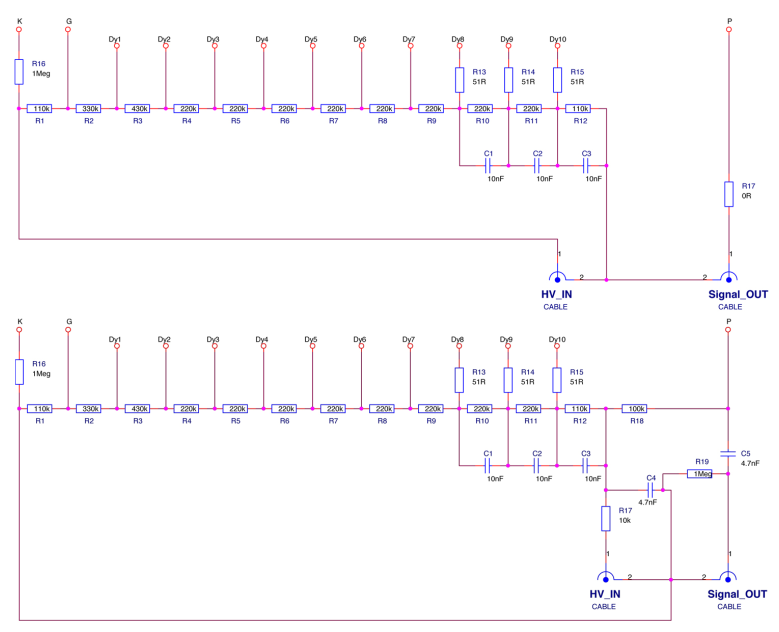
\includegraphics[scale=0.5]{3DesignPrinciples/32Tritium_detector/VoltageDividerPMT.png}
\caption{Hamamatsu commercial voltage divider electronic circuit. Upper circuit with negative supply and lower circuit with positive supply.\label{fig:VoltageDividerCircuit}~\cite{DataSheetPMTs}}
\end{figure}

%The electronic circuit that can be supplied with negative voltage is faster due to the ausence of the capacitances C4 and C5, but the other circuit, supplied with positive voltage, can be interesting for other tasks like the measurement of PMT currents. We will use both, depends on the objective of the study.

Focusing electrodes guide the photoelectrons to the first dinode. They have an collection efficiency (CE) defined as the ratio of the number of photoelectrons reaching the first dinode and the number of photoelectrons leaving the photocathode and its value is around $80\%$. The dynodes achieve the electron multiplication. A voltage difference between adjacent dynodes accelerates the electrons and produce their multiplication. The multiplication factor of each dynode, $\delta$, is commonly around 5 and is strongly dependent on the HV. If all dynodes have the same gain, the overall gain of a PMT with N dynodes is \cite{Knoll}:

\begin{equation}
G = CE\cdot{} \delta^N
\label{eq:PMTGain}
\end{equation}

that give an overall gain of a PMT of the order of $10^6$, strongly dependent on the applied HV.

The multiplication stage adds an uncertainty in the measurement. Working without gain allows to count the number of photons that reach the PMT. This can be done by short-circuiting all the dynodes and the anode and collecting the signal directly of the photocatode. This special setup was used for fiber characterization, described in section \ref{subsec:CharacterizationFibers}.

%Finally, the anode is the point where the collection of all the electrons produced takes place and it is the one that gives rise to the output signal of the PMTs.

\end{enumerate}

The output pulse of a PMT has a width of the order of tens of nanoseconds. The multiplication process can be described as a Poisson statistical process. For each electron in the first dynode, G new electrons are created with a variance of $\sqrt{G}$.

The output signal of a PMT is linear with the number of photons that reach its sensitive part up to a saturation limit, at which the linearity is lost. This limit depends on the PMT model.

The photocathode may emit electrons without any scintillation light. This signal is named dark current, $I_{DC}$, and can  arise due thermoionic emission and, for the PMTs used, this value is around $2~\nano\ampere$ according to their data sheet.

The characterization of the PMTs used for dark current, gain for several HV and quantum efficiency,  was done at IFIC in the framework of NEXT experiment \cite{CalibrationPMTsNEXT}. 